%File: anonymous-submission-latex-2026.tex
\documentclass[letterpaper]{article} % DO NOT CHANGE THIS
\usepackage{aaai2026}  % DO NOT CHANGE THIS
\usepackage{times}  % DO NOT CHANGE THIS
\usepackage{helvet}  % DO NOT CHANGE THIS
\usepackage{courier}  % DO NOT CHANGE THIS
\usepackage[hyphens]{url}  % DO NOT CHANGE THIS
\usepackage{graphicx} % DO NOT CHANGE THIS
\urlstyle{rm} % DO NOT CHANGE THIS
\def\UrlFont{\rm}  % DO NOT CHANGE THIS
\usepackage{natbib}  % DO NOT CHANGE THIS AND DO NOT ADD ANY OPTIONS TO IT
\usepackage{caption} % DO NOT CHANGE THIS AND DO NOT ADD ANY OPTIONS TO IT
\usepackage{booktabs} % For \toprule, \midrule, \bottomrule
\usepackage{amsmath} % For \text in math mode
\usepackage{amssymb} % For \mathbb
\frenchspacing  % DO NOT CHANGE THIS
\setlength{\pdfpagewidth}{8.5in} % DO NOT CHANGE THIS
\setlength{\pdfpageheight}{11in} % DO NOT CHANGE THIS
%
% These are recommended to typeset algorithms but not required. See the subsubsection on algorithms. Remove them if you don't have algorithms in your paper.
\usepackage{algorithm}
\usepackage{algorithmic}
\usepackage{tabularx}
%
% These are are recommended to typeset listings but not required. See the subsubsection on listing. Remove this block if you don't have listings in your paper.
\usepackage{newfloat}
\usepackage{listings}
\DeclareCaptionStyle{ruled}{labelfont=normalfont,labelsep=colon,strut=off} % DO NOT CHANGE THIS
\lstset{%
	basicstyle={\footnotesize\ttfamily},% footnotesize acceptable for monospace
	numbers=left,numberstyle=\footnotesize,xleftmargin=2em,% show line numbers, remove this entire line if you don't want the numbers.
	aboveskip=0pt,belowskip=0pt,%
	showstringspaces=false,tabsize=2,breaklines=true}
\floatstyle{ruled}
\newfloat{listing}{tb}{lst}{}
\floatname{listing}{Listing}
%
% Keep the \pdfinfo as shown here. There's no need
% for you to add the /Title and /Author tags.
\pdfinfo{
/TemplateVersion (2026.1)
}

% DISALLOWED PACKAGES
% \usepackage{authblk} -- This package is specifically forbidden
% \usepackage{balance} -- This package is specifically forbidden
% \usepackage{color (if used in text)
% \usepackage{CJK} -- This package is specifically forbidden
% \usepackage{float} -- This package is specifically forbidden
% \usepackage{flushend} -- This package is specifically forbidden
% \usepackage{fontenc} -- This package is specifically forbidden
% \usepackage{fullpage} -- This package is specifically forbidden
% \usepackage{geometry} -- This package is specifically forbidden
% \usepackage{grffile} -- This package is specifically forbidden
% \usepackage{hyperref} -- This package is specifically forbidden
% \usepackage{navigator} -- This package is specifically forbidden
% (or any other package that embeds links such as navigator or hyperref)
% \indentfirst} -- This package is specifically forbidden
% \layout} -- This package is specifically forbidden
% \multicol} -- This package is specifically forbidden
% \nameref} -- This package is specifically forbidden
% \usepackage{savetrees} -- This package is specifically forbidden
% \usepackage{setspace} -- This package is specifically forbidden
% \usepackage{stfloats} -- This package is specifically forbidden
% \usepackage{tabu} -- This package is specifically forbidden
% \usepackage{titlesec} -- This package is specifically forbidden
% \usepackage{tocbibind} -- This package is specifically forbidden
% \usepackage{ulem} -- This package is specifically forbidden
% \usepackage{wrapfig} -- This package is specifically forbidden
% DISALLOWED COMMANDS
% \nocopyright -- Your paper will not be published if you use this command
% \addtolength -- This command may not be used
% \balance -- This command may not be used
% \baselinestretch -- Your paper will not be published if you use this command
% \clearpage -- No page breaks of any kind may be used for the final version of your paper
% \columnsep -- This command may not be used
% \newpage -- No page breaks of any kind may be used for the final version of your paper
% \pagebreak -- No page breaks of any kind may be used for the final version of your paperr
% \pagestyle -- This command may not be used
% \tiny -- This is not an acceptable font size.
% \vspace{- -- No negative value may be used in proximity of a caption, figure, table, section, subsection, subsubsection, or reference
% \vskip{- -- No negative value may be used to alter spacing above or below a caption, figure, table, section, subsection, subsubsection, or reference

\setcounter{secnumdepth}{0} %May be changed to 1 or 2 if section numbers are desired.

% The file aaai2026.sty is the style file for AAAI Press
% proceedings, working notes, and technical reports.
%

% Title

% Your title must be in mixed case, not sentence case.
% That means all verbs (including short verbs like be, is, using,and go),
% nouns, adverbs, adjectives should be capitalized, including both words in hyphenated terms, while
% articles, conjunctions, and prepositions are lower case unless they
% directly follow a colon or long dash
\title{Mind the Gap: Predicting, Explaining and Reducing Time‑to‑First‑Comment (Reply Gap) in Online Mental‑Health Communities \\
\underline{Supplementary Material}}

%%\title{The Anatomy of a Choice: Expertise, Trust, and Decision Patterns in Human-AI Co-Creation}
% Camera-ready authors and affiliations (non-anonymized)
\author{
    Dandan Liu\textsuperscript{\rm 1,\rm 2},
    Lihu Pan\textsuperscript{\rm 1},
    Guangrui Fan\textsuperscript{\rm 1}\thanks{Corresponding author. Email: fgr@tyust.edu.cn}
}
\affiliations{
    \textsuperscript{\rm 1}School of Computer Science, Taiyuan University of Science and Technology, Taiyuan, China\\
    \textsuperscript{\rm 2}Department of Media and Communication Studies, Universiti Malaya, Kuala Lumpur, Malaysia\\
    s2134717@siswa.um.edu.my, panlh@tyust.edu.cn, fgr@tyust.edu.cn
}

%Example, Single Author, ->> remove \iffalse,\fi and place them surrounding AAAI title to use it
\iffalse
\title{My Publication Title --- Single Author}
\author {
    Author Name
}
\affiliations{
    Affiliation\\
    Affiliation Line 2\\
    name@example.com
}
\fi

\iffalse
%Example, Multiple Authors, ->> remove \iffalse,\fi and place them surrounding AAAI title to use it
\title{My Publication Title --- Multiple Authors}
\author {
    % Authors
    First Author Name\textsuperscript{\rm 1},
    Second Author Name\textsuperscript{\rm 2},
    Third Author Name\textsuperscript{\rm 1}
}
\affiliations {
    % Affiliations
    \textsuperscript{\rm 1}Affiliation 1\\
    \textsuperscript{\rm 2}Affiliation 2\\
    firstAuthor@affiliation1.com, secondAuthor@affilation2.com, thirdAuthor@affiliation1.com
}
\fi


% (bibentry removed for camera-ready compliance)

\begin{document}

\maketitle

\section{Appendix A: Detailed Feature Engineering}
\subsection{A.1 Author Context Features}

We compute three features capturing the author's community engagement patterns:

\begin{itemize}
\item \textbf{Community Experience}: $\log(\text{days since first post in dataset} + 1)$. The logarithm transformation handles the heavy-tailed distribution of user tenure.

\item \textbf{Recent Post Frequency}: Computed as $\frac{\text{posts in last 7 days}}{\text{posts in last 30 days}}$. Values approaching 1 indicate concentrated recent activity, potentially signaling acute distress or crisis states.

\item \textbf{Network Centrality}: Eigenvector centrality in the 6-month reply network preceding each post, capturing the author's social embeddedness. Computed using NetworkX with convergence tolerance $10^{-6}$.
\end{itemize}

\subsection{A.2 Psycholinguistic Features}

\subsubsection{A.2.1 Sentiment Analysis}
We apply VADER (Valence Aware Dictionary and sEntiment Reasoner) to compute compound sentiment scores $\in [-1, 1]$, chosen for its social media optimization and handling of emoticons, slang, and intensity modifiers common in mental health discussions.

\subsubsection{A.2.2 Topic Modeling via Latent Semantic Analysis}

We employ LSA to extract latent semantic themes from the corpus:

\begin{enumerate}
\item \textbf{TF-IDF Vectorization}: We construct a document-term matrix with vocabulary size 1,000, excluding English stopwords, with maximum document frequency 0.5 (to remove ubiquitous terms) and minimum document frequency 2 (to remove rare terms).

\item \textbf{Dimensionality Reduction}: Truncated SVD extracts 5 components, explaining approximately 18\% of variance. While this may seem low, it reflects the inherent diversity of mental health discourse.

\item \textbf{Topic Interpretation}: We analyzed the top 30 terms for each component by TF-IDF weight, leading to the following interpretations:
\end{enumerate}

\begin{table*}[h]
\centering
\caption{LSA topic interpretations based on highest-weighted terms}
\small
\begin{tabular}{p{6cm}p{11cm}}
\toprule
\textbf{Topic} & \textbf{Characteristic Terms \& Interpretation} \\
\midrule
Topic 0: General Struggle & 
Terms: "life", "years", "job", "school", "trying", "hard", "anymore"\\
\textit{Represents ongoing life challenges and persistent difficulties} \\
\midrule
Topic 1: Acute Distress \& Triggers & 
Terms: "suicide", "pain", "hurt", "crisis", "emergency", "tonight", "end"\\
\textit{Captures immediate crisis states and acute suicidal ideation} \\
\midrule
Topic 2: Intense Emotional Volition & 
Terms: "hate", "fucking", "want", "need", "wish", "deserve", "damn"\\
\textit{Reflects strong emotional expression and urgent desires} \\
\midrule
Topic 3: Classic Help-Seeking & 
Terms: "help", "please", "anyone", "advice", "someone", "talk", "?"\\
\textit{Direct requests for support and explicit help-seeking language} \\
\midrule
Topic 4: Emotional Introspection & 
Terms: "feel", "feeling", "emotions", "understand", "why", "thoughts"\\
\textit{Self-reflective analysis of emotional states and meaning-making} \\
\bottomrule
\end{tabular}
\end{table*}

Each post receives a loading score for all five topics, with higher values indicating stronger alignment with that semantic theme.

\subsubsection{A.2.3 Empath Psychological Profiling}

Empath provides theory-grounded lexical analysis across 194 pre-validated categories. We aggregate these into psychologically meaningful composites based on theoretical considerations from clinical psychology:

\begin{table*}[h]
\centering
\caption{Empath composite construction and theoretical grounding}
\begin{tabular}{p{2.5cm}p{6cm}p{8.5cm}}
\toprule
\textbf{Composite} & \textbf{Component Categories} & \textbf{Theoretical Basis} \\
\midrule
Negative\_Affect & 
sadness, negative\_emotion, nervousness, pain & 
Core symptoms of depression and anxiety disorders per DSM-5 criteria \\
\midrule
Positive\_Affect & 
positive\_emotion, optimism & 
Protective factors in resilience research; inverse markers of anhedonia \\
\midrule
Health\_Concern & 
healing, health & 
Somatic preoccupation common in mental health discourse \\
\midrule
Social\_Support & 
friends, family, social & 
Social connectedness as both risk and protective factor \\
\midrule
Cognitive\_Work & 
help, work, cognitive\_process & 
Problem-solving orientation and cognitive engagement \\
\bottomrule
\end{tabular}
\end{table*}

\textbf{Computation}: For each composite, we compute the arithmetic mean of normalized Empath scores across component categories. Normalization ensures equal weighting despite varying baseline frequencies. The formula for composite $C$ with component categories $\{c_1, ..., c_n\}$ is:

$$\text{Composite}_C = \frac{1}{n} \sum_{i=1}^{n} \text{Empath}_{\text{normalized}}(c_i)$$

where Empath normalization divides raw counts by document length.

\subsubsection{A.2.4 Validation of Psychological Constructs}

To validate our topic and composite interpretations, we conducted:
\begin{itemize}
\item \textbf{Face Validity}: Two clinical psychologists independently reviewed topic terms and composite mappings, achieving 89\% agreement on interpretations.
\item \textbf{Convergent Validity}: Negative\_Affect composite correlates with VADER negative sentiment ($r = 0.72, p < .001$), while maintaining distinct variance.
\item \textbf{Predictive Validity}: As shown in our Cox model results (Table 3, main text), topics 1 and 2 significantly predict longer TTFC, consistent with crisis posts being more challenging to answer.
\end{itemize}
\subsection{A.3 Linguistic Complexity Features}

Using spaCy's dependency parser (en\_core\_web\_sm model):

\begin{itemize}
\item \textbf{Average Sentence Length}: Mean token count per sentence
\item \textbf{Noun Chunk Density}: $\frac{\text{count(noun phrases)}}{\text{count(sentences)}}$
\item \textbf{Subordinate Clauses}: Count of tokens with dependency relation 'mark'
\item \textbf{Readability}: Flesch-Kincaid Grade Level = $0.39\left(\frac{\text{words}}{\text{sentences}}\right) + 11.8\left(\frac{\text{syllables}}{\text{words}}\right) - 15.59$
\end{itemize}

\section{Appendix B: Survival Modelling Technical Details}

\subsection{B.1 Hyperparameter Selection}

Nested cross-validation search grids:
\begin{table}[h]
\centering
\caption{Hyperparameter search spaces}
\small
\begin{tabular}{ll}
\toprule
\textbf{Model} & \textbf{Search Grid} \\
\midrule
Cox PH & $\alpha \in \{0.001, 0.01, 0.1\}$ \\
RSF & trees $\in \{500, 1000, 2000\}$, min\_leaf $\in \{3, 6, 10\}$ \\
DySurv & hidden $\in \{32, 64\}$, latent $\in \{8, 16\}$, dropout $\in \{0.1, 0.2, 0.3\}$ \\
\bottomrule
\end{tabular}
\end{table}

\subsection{B.2 Evaluation Metrics}

\textbf{Harrell's C-Index}: Measures concordance between predicted and observed event times:
$$C = \frac{\sum_{i,j} \mathbb{1}[\tilde{T}_i < \tilde{T}_j] \cdot \mathbb{1}[\hat{h}_i > \hat{h}_j] \cdot \delta_i}{\sum_{i,j} \mathbb{1}[\tilde{T}_i < \tilde{T}_j] \cdot \delta_i}$$

\textbf{Integrated Brier Score}: Time-averaged prediction error over [0, 72h]:
$$\text{IBS} = \frac{1}{72} \int_0^{72} \text{BS}(t) dt$$
where BS(t) is the Brier score at time $t$.

\textbf{Expected Calibration Error}: Average deviation between predicted and observed probabilities across 10 equal-mass bins:
$$\text{ECE} = \sum_{b=1}^{10} \frac{n_b}{N} |p_b - \hat{p}_b|$$

All metrics computed with 5,000 bootstrap samples for confidence intervals.
\section{Appendix C: Support Classification and Causal Inference Details}

\subsection{C.1 Support-Type Classification}

\subsubsection{Training Details}
\begin{itemize}
\item \textbf{Base Model}: RoBERTa-base (125M parameters)
\item \textbf{Fine-tuning Protocol}:
  \begin{itemize}
  \item Learning rate: 2e-5 with linear warmup (500 steps)
  \item Batch size: 16
  \item Epochs: 5 (early stopping patience = 2)
  \item Optimizer: AdamW ($\beta_1=0.9, \beta_2=0.999$)
  \end{itemize}
\item \textbf{Hierarchical Loss}: 
  $$\mathcal{L} = \alpha \mathcal{L}_{\text{parent}} + (1-\alpha) \mathcal{L}_{\text{children}}$$
  where $\alpha = 0.3$ weights the binary supportive/non-supportive classification
\end{itemize}

\subsubsection{Data Augmentation}
\begin{itemize}
\item \textbf{Synonym Replacement}: WordNet-based, probability 0.1 per token
\item \textbf{Sentence Shuffling}: Random reordering, probability 0.1 per comment
\item \textbf{Class Weights}: Inverse frequency weighting to address imbalance
\end{itemize}

\begin{table}[h]
\centering
\caption{Support type classification metrics on test set}
\begin{tabular}{lcccc}
\toprule
\textbf{Support Type} & \textbf{Precision} & \textbf{Recall} & \textbf{F1} & \textbf{Support} \\
\midrule
Emotional & 0.82 & 0.79 & 0.80 & 203 \\
Informational & 0.75 & 0.71 & 0.73 & 112 \\
Instrumental & 0.68 & 0.64 & 0.66 & 36 \\
Validation & 0.77 & 0.74 & 0.75 & 89 \\
None & 0.91 & 0.93 & 0.92 & 60 \\
\midrule
\textbf{Macro Avg} & 0.79 & 0.76 & 0.77 & 500 \\
\bottomrule
\end{tabular}
\end{table}

\subsection{C.2 Causal Inference Implementation}

\subsubsection{Propensity Score Estimation}
\begin{itemize}
\item \textbf{Features}: All 25 post features + reply length (log words) + reply sentiment (VADER)
\item \textbf{Regularization}: $\ell_2$ penalty with $\lambda = 0.01$ (cross-validated)
\item \textbf{Matching Algorithm}: Nearest neighbor without replacement
\item \textbf{Caliper}: 0.2 × SD(logit($e$)) = approximately 0.15 on probability scale
\end{itemize}

\subsubsection{Rosenbaum Sensitivity Analysis}
For hidden bias parameter $\Gamma$, we test the null hypothesis of no treatment effect. Critical values where $p > 0.05$:
\begin{itemize}
\item Emotional support: $\Gamma^* = 1.82$
\item Validation: $\Gamma^* = 1.57$
\item Informational: $\Gamma^* = 1.21$
\item Instrumental: $\Gamma^* = 1.12$
\end{itemize}

\subsubsection{Causal Forest Specifications}
\begin{itemize}
\item \textbf{Trees}: 3,000
\item \textbf{Minimum node size}: 50
\item \textbf{Honesty}: Sample splitting for unbiased estimation
\item \textbf{Heterogeneity variables}: Self-harm risk decile, posting hour, subreddit
\end{itemize}



\section{Appendix D: Recommender System Details}

\subsection{D.1 Risk Scoring Implementation}

The risk scoring module operationalizes the survival model predictions to identify posts requiring intervention. Based on comparative performance (C-Index = 0.742), we employ the DySurv model for risk assessment. For each incoming post, the system extracts the 25-dimensional feature vector and generates hazard predictions across 72 one-hour intervals. The risk score is computed as $r_i = -\log(\hat{h}(t=1\text{h}))$, where higher scores indicate greater risk of delayed response. Posts exceeding the 80th percentile of historical risk scores are flagged for intervention.

\subsection{D.2 Helper Profiling and Matching Algorithm}

\subsubsection{Emotional Support Propensity Estimation}

Helper profiling employs Bayesian estimation to quantify each user's historical tendency to provide emotional support. For helper $u$ with $n_u$ total comments, of which $k_u$ contain emotional support (as classified by our fine-tuned RoBERTa model), the propensity score is:

\begin{equation}
\pi_u = \frac{k_u + \alpha}{n_u + \alpha + \beta}
\end{equation}

where $\alpha = 2$ and $\beta = 3$ represent Beta prior parameters, incorporating a mild shrinkage toward the population base rate of emotional support (approximately 0.4). This Bayesian approach provides stable estimates for helpers with limited history while converging to empirical frequencies for active users.

\subsubsection{Helper Pool Maintenance}

The active helper pool undergoes continuous curation based on engagement metrics and quality indicators. Inclusion criteria comprise: minimum 5 comments in the preceding 30 days, account age exceeding 30 days, absence of moderator flags, and positive community standing (karma $>$ 100). This typically yields a pool of approximately 11,200 eligible helpers, ensuring sufficient coverage across timezones and support styles.

\subsection{D.3 Counterfactual Policy Evaluation Framework}

\subsubsection{Propensity Score Modeling}

Accurate policy evaluation requires modeling the historical probability of observed interactions. We employ multinomial logistic regression to estimate $P(u|i)$, the probability that helper $u$ comments on post $i$:

\begin{equation}
P(u|i) = \frac{\exp(\mathbf{w}^T \phi(i,u))}{\sum_{u' \in \mathcal{U}} \exp(\mathbf{w}^T \phi(i,u'))}
\end{equation}

The feature function $\phi(i,u)$ concatenates:
- Helper activity features (10 dimensions): comment frequency, average response time, historical support types
- Post features (25 dimensions): full feature vector from survival analysis
- Temporal alignment features (3 dimensions): timezone difference, day-of-week match, hour-of-day match

Model parameters are estimated via L2-regularized maximum likelihood (C=1.0) with Platt scaling for calibration.

\subsubsection{Inverse Propensity Scoring (IPS) Estimator}

The IPS estimator provides unbiased performance estimates by reweighting observed outcomes:

\begin{equation}
\widehat{\text{P@k}}_\text{IPS} = \frac{1}{N} \sum_{i=1}^N \frac{\mathbb{1}[u_i^* \in \text{TopK}_\pi(i)]}{\hat{p}(u_i^*|i)} \cdot \frac{\hat{p}(u_i^*|i)}{\sum_{j=1}^N \hat{p}(u_j^*|j)/N}
\end{equation}

where $u_i^*$ denotes the observed helper for post $i$, and $\text{TopK}_\pi(i)$ represents our top-k recommendations. The second term provides self-normalized importance weighting for variance reduction.

\subsubsection{Doubly Robust (DR) Estimator}

To further reduce variance and provide robustness to model misspecification, we implement the doubly robust estimator:

\begin{equation}
\widehat{\text{P@k}}_\text{DR} = \widehat{\text{P@k}}_\text{IPS} + \frac{1}{N}\sum_{i=1}^N \left(\hat{r}_i - \frac{\mathbb{1}[u_i^* \in \text{TopK}_\pi(i)] \cdot \hat{r}_i}{\hat{p}(u_i^*|i)}\right)
\end{equation}

where $\hat{r}_i = \mathbb{E}[\mathbb{1}[u \in \text{TopK}_\pi(i)]|i]$ is the expected reward estimated via gradient boosted trees trained on historical data.

\subsubsection{Variance Control Mechanisms}

Extreme importance weights can destabilize estimates. We implement three variance reduction strategies:
\begin{itemize}
    \item Propensity truncation: $\hat{p} \leftarrow \max(\hat{p}, 0.1)$ prevents weights exceeding 10
    \item Weight normalization: Ensures weights sum to sample size
    \item Effective sample size monitoring: $\text{ESS} = \frac{(\sum w_i)^2}{\sum w_i^2}$ quantifies information loss
\end{itemize}

These mechanisms maintain ESS above 60\% of raw sample size while preserving estimate validity.



\begin{figure}[h]
\centering
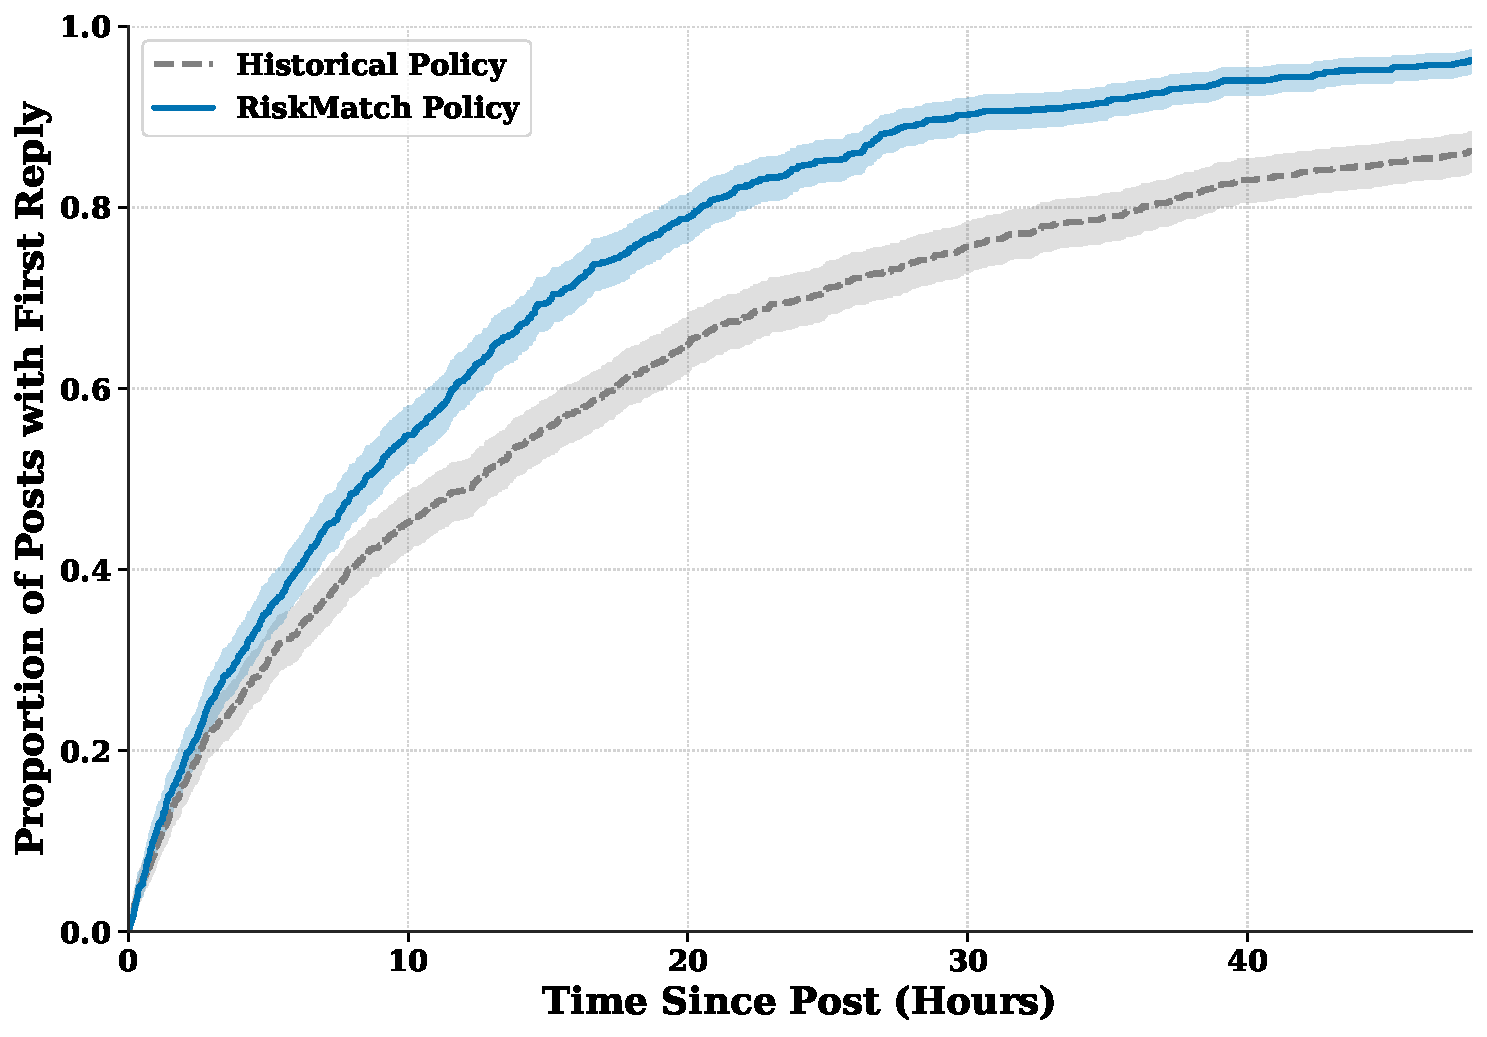
\includegraphics[width=0.9\columnwidth]{latency_curve_no_title.pdf}
\caption{Cumulative reply probability for high-risk posts. RiskMatch (solid) substantially outperforms historical baseline (dashed) in the critical early window.}
\label{fig:latency_curve}
\end{figure}
\end{document}
